\documentclass{standalone}
\usepackage{tikz}
\usetikzlibrary{patterns, positioning}
\usetikzlibrary{shapes.misc}
\usepackage[outline]{contour}
\contourlength{1.5pt} 


\begin{document}
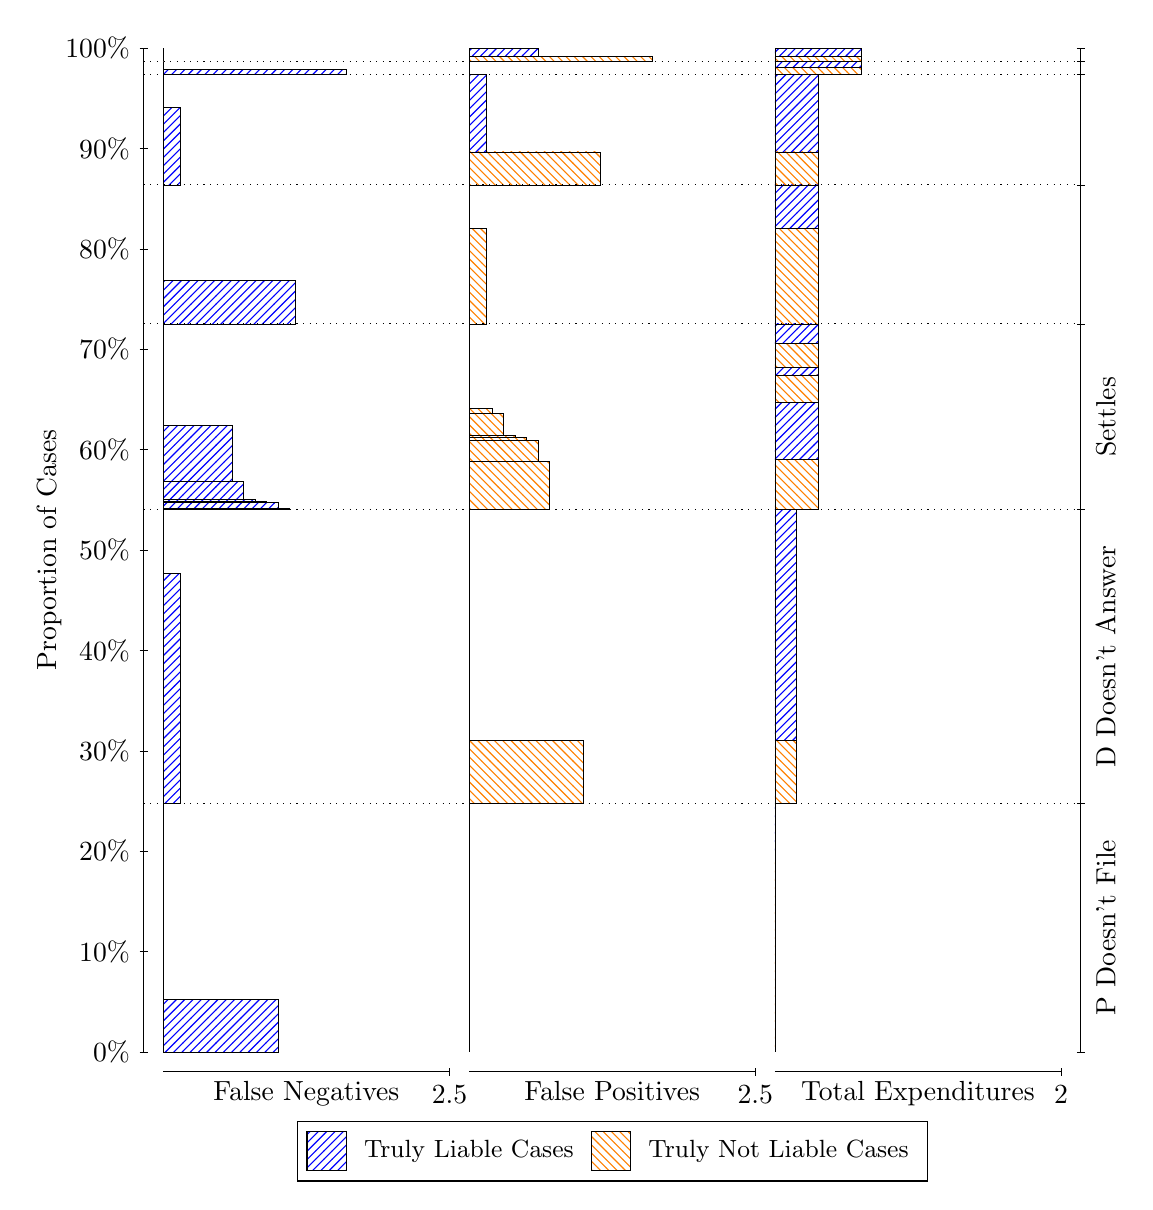
\begin{tikzpicture}
\draw[black, very thin] (1.5,1.75) -- (1.5,14.5);
\node[rotate=90, text=black, anchor=center] at (0.3, 8.125) {Proportion of Cases};
\draw[black, very thin] (1.45,1.75) -- (1.55,1.75);
\node[text=black, anchor=east] at (1.45, 1.75) {0\%};
\draw[black, very thin] (1.45,3.025) -- (1.55,3.025);
\node[text=black, anchor=east] at (1.45, 3.025) {10\%};
\draw[black, very thin] (1.45,4.3) -- (1.55,4.3);
\node[text=black, anchor=east] at (1.45, 4.3) {20\%};
\draw[black, very thin] (1.45,5.575) -- (1.55,5.575);
\node[text=black, anchor=east] at (1.45, 5.575) {30\%};
\draw[black, very thin] (1.45,6.85) -- (1.55,6.85);
\node[text=black, anchor=east] at (1.45, 6.85) {40\%};
\draw[black, very thin] (1.45,8.125) -- (1.55,8.125);
\node[text=black, anchor=east] at (1.45, 8.125) {50\%};
\draw[black, very thin] (1.45,9.4) -- (1.55,9.4);
\node[text=black, anchor=east] at (1.45, 9.4) {60\%};
\draw[black, very thin] (1.45,10.675) -- (1.55,10.675);
\node[text=black, anchor=east] at (1.45, 10.675) {70\%};
\draw[black, very thin] (1.45,11.95) -- (1.55,11.95);
\node[text=black, anchor=east] at (1.45, 11.95) {80\%};
\draw[black, very thin] (1.45,13.225) -- (1.55,13.225);
\node[text=black, anchor=east] at (1.45, 13.225) {90\%};
\draw[black, very thin] (1.45,14.5) -- (1.55,14.5);
\node[text=black, anchor=east] at (1.45, 14.5) {100\%};

\draw[black, very thin] (13.4,1.75) -- (13.4,14.5);
\draw[black, very thin] (13.35,1.75) -- (13.45,1.75);
\node[anchor=west] at (13.35, 1.75) {};
\draw[black, very thin] (13.35,4.9074) -- (13.45,4.9074);
\node[anchor=west] at (13.35, 4.9074) {};
\draw[black, very thin] (13.35,8.6361) -- (13.45,8.6361);
\node[anchor=west] at (13.35, 8.6361) {};
\draw[black, very thin] (13.35,10.996) -- (13.45,10.996);
\node[anchor=west] at (13.35, 10.996) {};
\draw[black, very thin] (13.35,12.762) -- (13.45,12.762);
\node[anchor=west] at (13.35, 12.762) {};
\draw[black, very thin] (13.35,14.166) -- (13.45,14.166);
\node[anchor=west] at (13.35, 14.166) {};
\draw[black, very thin] (13.35,14.326) -- (13.45,14.326);
\node[anchor=west] at (13.35, 14.326) {};
\draw[black, very thin] (13.35,14.5) -- (13.45,14.5);
\node[anchor=west] at (13.35, 14.5) {};

\draw[black, very thin, pattern color=blue, pattern=north east lines] (1.75,1.75) rectangle (3.2033,2.4182);
\draw[black, very thin, pattern color=orange, pattern=north west lines] (1.75,2.4182) rectangle (1.75,4.9074);
\draw[black, very thin, pattern color=blue, pattern=north east lines] (1.75,4.9074) rectangle (1.968,7.8329);
\draw[black, very thin, pattern color=orange, pattern=north west lines] (1.75,7.8329) rectangle (1.75,8.6361);
\draw[black, very thin, pattern color=blue, pattern=north east lines] (1.75,8.6361) rectangle (3.3487,8.6515);
\draw[black, very thin, pattern color=blue, pattern=north east lines] (1.75,8.6515) rectangle (3.2033,8.7304);
\draw[black, very thin, pattern color=blue, pattern=north east lines] (1.75,8.7304) rectangle (3.058,8.7427);
\draw[black, very thin, pattern color=blue, pattern=north east lines] (1.75,8.7427) rectangle (2.9127,8.7704);
\draw[black, very thin, pattern color=blue, pattern=north east lines] (1.75,8.7704) rectangle (2.7673,8.9937);
\draw[black, very thin, pattern color=blue, pattern=north east lines] (1.75,8.9937) rectangle (2.622,9.7086);
\draw[black, very thin, pattern color=orange, pattern=north west lines] (1.75,9.7086) rectangle (1.75,10.996);
\draw[black, very thin, pattern color=blue, pattern=north east lines] (1.75,10.996) rectangle (3.4213,11.549);
\draw[black, very thin, pattern color=orange, pattern=north west lines] (1.75,11.549) rectangle (1.75,12.762);
\draw[black, very thin, pattern color=blue, pattern=north east lines] (1.75,12.762) rectangle (1.968,13.746);
\draw[black, very thin, pattern color=orange, pattern=north west lines] (1.75,13.746) rectangle (1.75,14.166);
\draw[black, very thin, pattern color=blue, pattern=north east lines] (1.75,14.166) rectangle (4.0753,14.233);
\draw[black, very thin, pattern color=orange, pattern=north west lines] (1.75,14.233) rectangle (1.75,14.326);
\draw[black, very thin, pattern color=orange, pattern=north west lines] (1.75,14.326) rectangle (1.75,14.396);
\draw[black, very thin, pattern color=blue, pattern=north east lines] (1.75,14.396) rectangle (1.75,14.5);
\draw[black, very thin, pattern color=orange, pattern=north west lines] (5.6333,1.75) rectangle (5.6333,4.2391);
\draw[black, very thin, pattern color=blue, pattern=north east lines] (5.6333,4.2391) rectangle (5.6333,4.9074);
\draw[black, very thin, pattern color=orange, pattern=north west lines] (5.6333,4.9074) rectangle (7.0867,5.7106);
\draw[black, very thin, pattern color=blue, pattern=north east lines] (5.6333,5.7106) rectangle (5.6333,8.6361);
\draw[black, very thin, pattern color=orange, pattern=north west lines] (5.6333,8.6361) rectangle (6.6507,9.2497);
\draw[black, very thin, pattern color=orange, pattern=north west lines] (5.6333,9.2497) rectangle (6.5053,9.5143);
\draw[black, very thin, pattern color=orange, pattern=north west lines] (5.6333,9.5143) rectangle (6.36,9.5519);
\draw[black, very thin, pattern color=orange, pattern=north west lines] (5.6333,9.5519) rectangle (6.2147,9.5766);
\draw[black, very thin, pattern color=orange, pattern=north west lines] (5.6333,9.5766) rectangle (6.0693,9.8617);
\draw[black, very thin, pattern color=orange, pattern=north west lines] (5.6333,9.8617) rectangle (5.924,9.9238);
\draw[black, very thin, pattern color=blue, pattern=north east lines] (5.6333,9.9238) rectangle (5.6333,10.996);
\draw[black, very thin, pattern color=orange, pattern=north west lines] (5.6333,10.996) rectangle (5.8513,12.209);
\draw[black, very thin, pattern color=blue, pattern=north east lines] (5.6333,12.209) rectangle (5.6333,12.762);
\draw[black, very thin, pattern color=orange, pattern=north west lines] (5.6333,12.762) rectangle (7.3047,13.181);
\draw[black, very thin, pattern color=blue, pattern=north east lines] (5.6333,13.181) rectangle (5.8513,14.166);
\draw[black, very thin, pattern color=orange, pattern=north west lines] (5.6333,14.166) rectangle (5.6333,14.259);
\draw[black, very thin, pattern color=blue, pattern=north east lines] (5.6333,14.259) rectangle (5.6333,14.326);
\draw[black, very thin, pattern color=orange, pattern=north west lines] (5.6333,14.326) rectangle (7.9587,14.396);
\draw[black, very thin, pattern color=blue, pattern=north east lines] (5.6333,14.396) rectangle (6.5053,14.5);
\draw[black, very thin, pattern color=orange, pattern=north west lines] (9.5167,1.75) rectangle (9.5167,4.2391);
\draw[black, very thin, pattern color=blue, pattern=north east lines] (9.5167,4.2391) rectangle (9.5167,4.9074);
\draw[black, very thin, pattern color=orange, pattern=north west lines] (9.5167,4.9074) rectangle (9.7892,5.7106);
\draw[black, very thin, pattern color=blue, pattern=north east lines] (9.5167,5.7106) rectangle (9.7892,8.6361);
\draw[black, very thin, pattern color=orange, pattern=north west lines] (9.5167,8.6361) rectangle (10.062,9.2743);
\draw[black, very thin, pattern color=blue, pattern=north east lines] (9.5167,9.2743) rectangle (10.062,10.002);
\draw[black, very thin, pattern color=orange, pattern=north west lines] (9.5167,10.002) rectangle (10.062,10.349);
\draw[black, very thin, pattern color=blue, pattern=north east lines] (9.5167,10.349) rectangle (10.062,10.443);
\draw[black, very thin, pattern color=orange, pattern=north west lines] (9.5167,10.443) rectangle (10.062,10.745);
\draw[black, very thin, pattern color=blue, pattern=north east lines] (9.5167,10.745) rectangle (10.062,10.996);
\draw[black, very thin, pattern color=orange, pattern=north west lines] (9.5167,10.996) rectangle (10.062,12.209);
\draw[black, very thin, pattern color=blue, pattern=north east lines] (9.5167,12.209) rectangle (10.062,12.762);
\draw[black, very thin, pattern color=orange, pattern=north west lines] (9.5167,12.762) rectangle (10.062,13.181);
\draw[black, very thin, pattern color=blue, pattern=north east lines] (9.5167,13.181) rectangle (10.062,14.166);
\draw[black, very thin, pattern color=orange, pattern=north west lines] (9.5167,14.166) rectangle (10.607,14.259);
\draw[black, very thin, pattern color=blue, pattern=north east lines] (9.5167,14.259) rectangle (10.607,14.326);
\draw[black, very thin, pattern color=orange, pattern=north west lines] (9.5167,14.326) rectangle (10.607,14.396);
\draw[black, very thin, pattern color=blue, pattern=north east lines] (9.5167,14.396) rectangle (10.607,14.5);
\draw[black, dotted] (1.5,4.9074) -- (13.4,4.9074);
\draw[black, dotted] (1.5,8.6361) -- (13.4,8.6361);
\draw[black, dotted] (1.5,10.996) -- (13.4,10.996);
\draw[black, dotted] (1.5,12.762) -- (13.4,12.762);
\draw[black, dotted] (1.5,14.166) -- (13.4,14.166);
\draw[black, dotted] (1.5,14.326) -- (13.4,14.326);
\draw[black, very thin] (1.75,1.5) -- (5.3833,1.5);
\node[text=black, anchor=north] at (3.5667, 1.5) {False Negatives};
\draw[black, very thin] (5.3833,1.45) -- (5.3833,1.55);
\node[text=black, anchor=north] at (5.3833, 1.45) {2.5};

\draw[black, very thin] (5.6333,1.5) -- (9.2667,1.5);
\node[text=black, anchor=north] at (7.45, 1.5) {False Positives};
\draw[black, very thin] (9.2667,1.45) -- (9.2667,1.55);
\node[text=black, anchor=north] at (9.2667, 1.45) {2.5};

\draw[black, very thin] (9.5167,1.5) -- (13.15,1.5);
\node[text=black, anchor=north] at (11.333, 1.5) {Total Expenditures};
\draw[black, very thin] (13.15,1.45) -- (13.15,1.55);
\node[text=black, anchor=north] at (13.15, 1.45) {2};

\node[text=black, centered, rotate=90] at (13.72, 3.3287) {\contour{white}{P Doesn't File}};
\node[text=black, centered, rotate=90] at (13.72, 6.7717) {\contour{white}{D Doesn't Answer}};
\node[text=black, centered, rotate=90] at (13.72, 9.8162) {\contour{white}{Settles}};





\draw (7.449999999999999,1.5) node[draw=none] (baseCoordinate) {};
\begin{scope}[align=center]
        \matrix[scale=0.5, draw=black, below=0.5cm of baseCoordinate, nodes={draw}, column sep=0.1cm]{
            \node[rectangle, draw, minimum width=0.5cm, minimum height=0.5cm, pattern color=blue, pattern=north east lines] {}; &
            \node[draw=none, font=\small, text=black] (B) {Truly Liable Cases}; &
            \node[rectangle, draw, minimum width=0.5cm, minimum height=0.5cm, pattern color=orange, pattern=north west lines] {}; &
            \node[draw=none, font=\small, text=black] (B) {Truly Not Liable Cases}; \\
            };
\end{scope}

\end{tikzpicture}
\end{document}